% !TEX encoding = UTF-8 Unicode
\documentclass[10pt,twocolumn,letterpaper]{article}

\usepackage[utf8]{inputenc}
\usepackage[T1]{fontenc}
\usepackage{textcomp,gensymb}
\usepackage{ae,aecompl}

\usepackage[english]{babel}
\usepackage[none]{hyphenat}

\usepackage{cvpr}
\usepackage{times}
\usepackage{epsfig,graphicx}
\usepackage{amsmath,amssymb}

\usepackage{enumitem}
\setlist{nosep}

\usepackage{multirow}

% Include other packages here, before hyperref.

% If you comment hyperref and then uncomment it, you should delete
% egpaper.aux before re-running latex.  (Or just hit 'q' on the first latex
% run, let it finish, and you should be clear).
\usepackage[breaklinks=true,bookmarks=false,hidelinks=true]{hyperref}

\cvprfinalcopy

%\def\cvprPaperID{****} % *** Enter the CVPR Paper ID here
%\def\httilde{\mbox{\tt\raisebox{-.5ex}{\symbol{126}}}}

\setcounter{page}{1}
\begin{document}

\title{XXXXXXXXXXXXXXXXXXXXXXXXXXXXXXXXXXX}

\author{Nicolò Bertozzi\\
S276406\\
{\tt\small nicolo.bertozzi@studenti.polito.it}
\and
Francesco Bianco Morghet\\
S277910\\
{\tt\small s277910@studenti.polito.it}
}

\maketitle
%\thispagestyle{empty}


\begin{abstract}
	In this work, we will explore a number of methods for tackling the action recognition task in the first person point of view. Starting from Ego-RNN, we will first experiment the effectiveness and the limits of the attention mechanism when applied on RGB frames; we will also evaluate the temporal network applied on warped optical flow frames and the two-stream approach proposed in Ego-RNN. Then, we will explore the power of an IDT-based self supervised task when added to the RGB network. Finally, we will try to replicate the promising results achieved by the RGB network on colorised warped optical flow frames by introducing a colorising block, WFCNet; after that, we will also propose a double input network capable of jointly handling RGB frames and colorised warped optical flow frames.
\end{abstract}


\section{Introduction}

One of the main challenges in the field of Computer Vision and Artificial Intelligence lies in the recognition of the actions included inside a video. Until now, the research has been concentrated on the data provided by specific kinds of cameras, used in particular areas and in particular places, which capture the alternating of the everyday life from an external narrator point of view, i.e in third person.

A lot of areas are interested in a classification based on first person videos. Among them, the robotic applications could be surely cited, ranging from the definition of the androids’ intelligence like iCub\textsuperscript{\textcopyright} to the autonomous driving. Other instances are surveillance; the composition of the people’s behavioural profiles, in order to predict and then to prevent potential offences; the analysis of the users’ content information to track their preferences and loyalize their experience inside a service; etc.

The datasets which contain this information have been very small until now, but this limit could be easily surpassed in the future with the growing increase of the sale of wearable devices, with the undeterred increment of the ease to have cameras at our disposal, and with the exponential growth of the number of photos and videos taken every day all over the world. 

In addition, first person images present further difficulties than the ones in third person. First of all, it is very frequent to observe part of the subject who is capturing the action in the video frame: this feature has to be used as a way of promoting the action recognition, and should not be a disadvantage for it. Then it is very probable that the camera which is taking the video is mounted on the head of the subject who is performing the operation, and therefore also the perspective change basing on what the cameraman is watching at that moment has to be taken into account.

Dependently on the context, the video classification could be more precise or less precise. A general purpose recognition can be reduced to a simple verb, but it would define the action in progress with subpar accuracy. Instead, a more careful recognition is composed of a verb plus a noun: in fact \emph{open}, \emph{open a door} or \emph{open a jar} are completely different actions.

\section{Related works}

In this section we introduce some of the recent approaches used to process first person videos along with some of the employed preprocessing techniques.

\subsection{Optical flow and warped optical flow}

In order to encode motion of objects and isolate it from their appearance, optical flow is often employed in many machine learning approaches.

The main assumption of the optical flow extraction procedure is that, between two still frames, objects have moved by a small amount, if any, and their brightness has not changed. This is not always true: for instance, an object could fall inside the shadow cast by another object, therefore altering their brightness. Formally, by writing the brightness $I$ as function of space $x,y$ and time $t$, the following equation can be expressed:
${I(x,y,t) = I(x + \Delta x, y + \Delta y, t + \Delta t)}$. By rewriting the right member as its Taylor expansion up to its first term, the following holds: $\nabla I \cdot \vec{V} = -I_t$. In this single equation, both the $x$ component and the $y$ component of velocity $V$ are unknown. This is described as the aperture problem, and so, to actually compute the optical flow, further constraints are put in place.

A main issue with optical flow is that camera motion highly influences the process, thus adding unnecessary noise to the computed results. So, in order to subtract camera motion, in \cite{wang2013trajectiories} the warped optical flow is introduced. It consists in inferring the global background motion by estimating the homography matrix and then subtracting the camera motion from the computed optical flow. This second procedure is particularly useful for removing noisy movements in the first person point of view videos, as in the case of an action cam mounted on a shoulder of a person.

\subsection{Two-stream approach}
\label{par:Ego-RNN}

The first person action recognition task has been tackled by several works in recent years, and various solutions involving deep learning algorithms have been proposed.

In \cite{Ego-RNN}, a ResNet-34, is used to extract feature embeddings from RGB images; then, a Convolutional Long Short-Term Memory (ConvLSTM) is used to model the temporal dependencies between the feature maps extracted by the convolutional segment and the spatial correlations inside each of those; finally, a linear classifier on the features extracted by the ConvLSTM is used to classify the portrayed action.

However, the aforementioned RGB network focuses on the appearances of each single frame, but it fails to take into account the motion happening in those frames in a effectively manner. To tackle this problem, a separate convolutional neural network can be trained on optical flows images; in \cite{Ego-RNN}, a ResNet-34 trained on warped optical flow images achieves better results than training on optical flow thanks to the compensation of camera motion of the former.

Then, on top of these two trained networks, a linear classifier is used to determine the class label of the given sample: while the classifier is trained on the output features of the two networks, also the two networks are fine tuned.

The main disadvantage of this two-stream approach is that motion information and appearance information are decoupled, since they are treated in two separate networks, hence any correlations among the two are not taken into account.

There exist however an attempts to go beyond the two streams approach and to deal with both appearance and motion in a single network by using an auxiliary task, as in the case of \cite{planamente2020joint} where a motion segmentation task is deployed.

\subsection{Attention model}
\label{par:AttentionModel}
One milestone for the development of a working solution for recognising the involved action is the acknowledgement of the important role played by the motion of the hands and the appearance of the objects in the scene. So, focusing the attention on the most important region of a frame of a video, while at the same time discarding irrelevant information, can be a key component for getting a great performance gain in terms of accuracy. For this reason, in \cite{Ego-RNN} an attention mechanism is employed in the ResNet backbone in order to extract features with spatial attention.

To extract features with spatial attention $f_{SA}$, \textit{class activation maps} (CAMs) are employed:
\begin{enumerate}
	\item The $l$ output feature maps of the very last convolutional layer of the backbone are forwarded to an average pool that reduces each feature map size to a 1x1 block, then those reduced feature maps are forwarded to a fully connected layer;
	\item The CAM for class $c$ is obtained, for each spatial location $i$, by dot multiplying the values of the $l$ feature maps at location $i$ and the weights of the neuron of the fully connected layer of class $c$, i.e. ${\text{CAM}_c(i) = \sum_l w_l^c f_l(i)}$. 
	\item The features with spatial attention $f_{SA}$ are obtained by performing the Hadamard product between the output feature maps of the very last convolutional layer of the backbone and the output of the softmax operation applied to the CAM of the class with the highest probability.
\end{enumerate}

To summarise, we can think of a CAM as the result of a linear classifier: given a spatial location, it outputs a score which states the relevance of that spatial location for the recognition of the performed action; by applying the softmax operation on the scores of all the spatial locations of the input, these scores can be turned into normalised scores (or probabilities) regarding how much each position is relevant for the action; then, by dot multiplying the normalised scores and input, the interesting regions of the input are amplified. The main reasoning behind this procedure is that the same classifier can also be used to discriminate the involved action: so by grouping a number of these linear classifiers in a fully connected layer and by feeding this fully connected layer with an average-pooled version of the input, a different neuron will reach the highest score depending on the depicted action; therefore, by computing the CAM using the weights of the neuron of the winning class, action-specific regions of the input frame are highlighted. However, we verified that this is not the case: by replicating the experiments proposed in \cite{Ego-RNN}, and also by running their trained model published online, we verified that, at convergence, the same hidden neuron is activated for all the input samples. As a result, we propose a simpler attention mechanism which is still capable of reaching the same performances.

%The limit of the attention mechanism applied on RGB images is that it does not take into account motion information, but it focuses on the appearance of each single frame in a stateless manner. So, despite the deployment of the attention mechanism, in \cite{Ego-RNN} in order to reach state of the art performances, a separate convolutional neural network is trained on stacked warp flow images, and then, a linear classifier is put on top of the output features of the two networks.

\subsection{Motion segmentation task}
\label{par:ms_task}
The main idea behind this procedure is the addition of an auxiliary task: given an architecture where first a convolutional neural network extracts feature embeddings from RGB frames and then a ConvLSTM models temporal and infra-spatial correlations of such features, a second task is added to the output of the convolutional neural network with the intention of helping this shared backbone to extract more meaningful features and taking motion into account as well.

In \cite{planamente2020joint}, a motion segmentation task is proposed. To do so, an \textit{improved dense trajectory} (IDT) is associated to each frame; basically, an IDT is a binary map that compensates for camera motion and that, for each pixel, states whether a moving keypoint is present or not. This motion map is used as a ground truth for a motion segmentation task: the output feature maps of the last convolutional layer of the shared backbone are forwarded to a second branch where they are first processed by a convolutional layer and then forwarded to a fully connected layer. This auxiliary task aims to minimise the pixel-by-pixel cross entropy loss between the predicted motion map and the ground truth. Both auxiliary task and main task are trained together, because the role of the auxiliary task is to help the shared backbone to extract better features, in the sense that they are able to take into account motion as well: for this reason, the losses of the auxiliary task and the main task are summed together during training.


\section{Proposed method}
Our method consists in first replacing the attention mechanism in the RGB network proposed in \cite{Ego-RNN} with a simpler but still equally effective one, which consists in just a linear classifier. After proving that this modified network achieves the same performances on RGB images, we try to leverage the strength of this network on warped optical flow frames. In order to adapt the warp flow frames to the RGB network, we perform a colorisation: to do so, we draw inspiration from \cite{carlucci2017de2}, where a convolutional neural network is used to colorise depth images. Finally, we propose a second variant where both RGB images and flow images are processed in a single network, which tries to model both the motion cues encoded by the warp flow frames, and the appearances of the objects encoded by the RGB frames.

\subsection{New attention mechanism}
\label{par:new_am}

As anticipated in \ref{par:AttentionModel}, the attention mechanism can be thought as a linear classifier that gives a relevance score for each spatial location of the input and then amplifies the relevant spatial locations of the input according to their scores. Therefore, we implement this variant on the RGB network proposed in \cite{Ego-RNN}.

The output feature maps of the last convolutional layer of the backbone, whose size is 512x7x7, is our input: there are 49 spatial locations and each one is described by 512 variables. A linear classifier, which is a simple 512 long vector, produces the relevance score for each of the 49 spatial locations; then, the softmax function is applied on the output scores, producing what can be referred to as activation map. Finally, the features with spatial attention $f_{SA}$ are obtained by performing the element-wise product of the input features and the activation map.

To put formally, given the input $f$ and $w$ the weights of the attention mechanism, the output score $s$ for the spatial location $i$ is given by ${s(i) = \sum_l w_l f_l(i)}$; the activation map $AM$ for spatial location $i$ is then computed as ${AM(i) = \frac{e^{s(i)}}{\sum_i e^{s(i)}}}$. The features with spatial attention $f_{SA}$ are then obtained by computing the element-wise product between the input $f$ and the activation map $AM$: ${f_{SA} = AM \odot f}$.

By placing this simplified attention mechanism in the RGB network proposed in \cite{Ego-RNN} (briefly described in \ref{par:Ego-RNN}), we will show that roughly the same performances are achieved.

\subsection{Warp flow colorisation}

The employment of optical flow has been proved to be effective in many machine learning applications as a tool to capture and effectively encode motion cues from moving objects. In this work, the warped optical flow is used since, as it has been introduced in the paragraphs above, it enables the compensation of camera movements, which is a great factor to take into account in first person videos.

So, the employed method can be decomposed into two main steps, which are briefly presented here and will be discussed in more details in the following paragraphs:
\begin{enumerate}
	\item A convolutional neural network, which performs the warp flow colorisation and will be referred to as WFCNet from this point on, is trained so that a mapping between warp flow frames and generated RGB frames is learnt; 
	\item Using WFCNet for inferring RGB frames from warp flow frames, a deep neural network consisting in a convolutional backbone, a ConvLSTM, an average pooling layer and a final fully connected layer is trained in a multi stage manner. We also propose a two stream variant, which consists in a shared backbone, fed with both colorised warp flow frames and original RGB frames.
\end{enumerate}

\subsubsection{WFCNet}

\begin{figure*}
	\begin{center}
		\includegraphics[width=\textwidth]{schemi/WFCNet_img.pdf}		
	\end{center}
	\caption{WFCNet module representation along with the whole architecture used in the training phase}
	\label{fig:WFCNet}
\end{figure*}

WFCNet is a ResNet-like network: it makes use of residual blocks which introduce additional direct connections from input to output that skip convolutional layers. This procedure enables a better gradient flow in the backward propagation step and prevents the gradient vanishing problem that limits the deepness of neural networks.

WFCNet is made of basic blocks; each block consists in: two convolutional layers with kernel size of 3, stride of 1 and padding of 1; one ReLu between them; batch normalisation at the output of each convolutional layer; a direct connection from input to output, which is obtained by summing the input of the block to the output of the second convolution.
As suggested by the work presented in \cite{springenberg2014striving}, the downsampling of the residual input is done by using a convolutional filter instead of a simple average pooling: in this way, an embedding can be learnt leading to better downsampled feature maps, while at the same time the advantages of the residual block are preserved.
The upsampling of the residual input is performed instead by applying a nearest neighbour resizing followed by a convolution filter with a stride 1 and kernel size of 1.

These basic blocks are grouped together in blocks that we can call macro blocks. It should be noted that the downsampling or upsampling are performed only by the first convolutional layer of each macro block. The downsampling is the result of the adoption of a convolution with a stride of 2, kernel size of 3 and padding of 1; on the other hand, the upsampling is performed using a nearest neighbour resizing followed by a convolutional filter with a stride 1, kernel size of 3 and padding of 1 on every side. 

This structure with gradual downsampling followed by a gradual upsampling allows the extraction of RGB images with semantic segmentation for hands and objects involved in the action, while at the same time all the other still objects are discarded and melted with the background. In this work, the transposed convolution for upsampling is not employed because its introduction resulted in repeating patterns in the output RGB frames that would not disappear even after many epochs of training: instead the employment of nearest neighbour for upsampling leads to better segmented images, which in turn leads to better overall results.

Finally, the output RGB frames of WFCNet are normalised: first the Sigmoid function is applied to every output value in order to get values in the $[0; 1]$ range; then, every channel of each pixel is normalised on the means and standard deviations of ImageNet, which are \texttt{mean=[0.485, 0.456, 0.406]}, \texttt{std=[0.229, 0.224, 0.225]}. The introduction of this block improves the performances of the model and its stability at the beginning of the training because, in the overall training procedure of this network, a ResNet-34 pre-trained on ImageNet is employed. Also, since WFCNet is later employed to colorise frames which are then fed to an RGB network whose backbone is pre-trained on ImageNet, it is important that those generated images are normalised in the correct manner in order to achieve optimal results. By explicitly introducing this block, we can be sure that the generated images meet this requirement.

\begin{table}
	\begin{tabular}{l|lp{40mm}}
	Conv 0 & CONV & 2x7x7x8, s=2, p=3 \\
	
	\hline
	\multirow{6}{*}{\shortstack{Conv 1\\(x2)}} & CONV & 8x3x3x8, s=1, p=1 \newline (s=2 for 1st block) \\
	& BN & \\
	& RELU & \\
	& CONV & 8x3x3x8, s=1, p=1 \\
	& BN & \\
	& RES & \\
	
	\hline
	\multirow{6}{*}{\shortstack{Conv 2\\(x3)}} & CONV & 16x3x3x16, s=1, p=1 \newline (8x3x3x16, s=2 for 1st block) \\
	& BN & \\
	& RELU & \\
	& CONV & 16x3x3x16, s=1, p=1 \\
	& BN & \\
	& RES & \\
	
	\hline
	& UPSAMPLE & factor=2 \\
	& CONV & 16x1x1x16, s=1, p=0 \\
	
	\hline
	\multirow{6}{*}{\shortstack{Deconv 1\\(x3)}} & CONV & 16x3x3x16, s=1, p=1 \\
	& BN & \\
	& RELU & \\
	& CONV & 16x3x3x16, s=1, p=1 \\
	& BN & \\
	& RES & \\
	
	\hline
	& UPSAMPLE & factor=2 \\
	& CONV & 16x1x1x16, s=1, p=0 \\
	
	\hline
	\multirow{6}{*}{\shortstack{Deconv 2\\(x2)}} & CONV & 8x3x3x8, s=1, p=1 \newline (16x3x3x8, for 1st block) \\
	& BN & \\
	& RELU & \\
	& CONV & 8x3x3x8, s=1, p=1 \\
	& BN & \\
	& RES & \\
	
	\hline
	\multirow{2}{*}{  Out} & CONV & 8x1x1x3, s=1, p=1 \\
	& NORM & \\
	
\end{tabular}
	\vspace{5mm}
	\label{tab:wfcnet}
	\caption{WFCNet detailed structure}
\end{table}

\subsubsection{Training WFCNet}
\label{par:TrainingWFCNet}

The aim of the WFCNet block is to learn a mapping from input warp flow frames to output RGB frames.

We propose two variants for WFCNet, which differ in the kind of input they accept:
\begin{enumerate}
	\item One single warp flow frame, consisting in two channel, i.e. the x-axis displacement and the y-axis displacement;
	\item A stack of five consecutive warp flow frames, which account to a total number of 10 channels.
\end{enumerate}

In order to train WFCNet, a ResNet-34, followed by an average pooling and a fully connected layer, are employed. The complete architecture is represented in figure \ref{fig:WFCNet}: the input frame is colorised by WFCNet; then the resulting RGB image is fed to the ResNet-34; finally, the output features of the ResNet-34 are forwarded to the classification block, which consists in an average pooling (which reduces the feature maps from a 512x7x7 volume to a vector of 512 elements) and a fully connected layer.

Each video sample consists in possibly more than one input frame, accounting for different time steps: for this reason, for each sample, multiple input frames are forwarded to the network, multiple RGB images are generated and so multiple output scores are produced by the final fully connected layer. For this reason, the average of the output scores is computed with respect to the time dimension.

We treat this task as a classification problem, where the aim of the whole architecture (consisting in WFCNet, ResNet, and classification block) is to predict the class label of the sample. For this reason, the \textit{Cross Entropy Loss} is employed, which can be expressed as ${L = -\sum_i^N{\log(P(y_i | x_i, w))}}$, where $N$ is the total number of samples, $x_i$ is the input sample, $y_i$ is the true label, and ${P(y_i | x_i, w)}$ is the predicted probability for the true label $y_i$ given the sample $x_i$ and the weights of the network $w$. The normalised probabilities for the different classes are computed using the softmax function: ${P(y_i | x_i, w) = \frac{e^{f_{y_i}}}{\sum_i e^{f_i}}}$.

The whole training procedure consists in two main stages:
\begin{enumerate}
	\item The ResNet-34 is pre-trained on ImageNet and its weights are kept frozen; the weights of WFCNet are randomly initialised using the uniform distribution according to the Kaiming procedure described in \cite{he2015delving}. Only WFCNet and the final fully connected layer are trained;
	\item In this second stage, besides fine tuning the weights of WFCNet and the final fully connected layer, also the weights of the very last ``macro block'' of the ResNet-34 are fine tuned: in this way, the performances of the whole architecture are improved.
\end{enumerate}
It should be noted that the performances of this architecture are not interesting \textit{per se}, since we are only interested in later reusing the WFCNet block in another network better suited for the action recognition task, i.e. the RGB network. However, we qualitatively observed to be present a positive correlation between high performances of this architecture and high performances of WFCNet in conjunction with the RGB network: so we employ this multi stage training for this particular reason.

\subsection{RGB network}
\label{par:our_rgb_network}

\begin{figure*}
	\begin{center}
		\includegraphics[width=\textwidth]{schemi/single_stream_img.pdf}		
	\end{center}
	\caption{Single-stream RGB network}
	\label{fig:SingleStream}
\end{figure*}

The single-stream RGB network is closely inspired by the RGB network proposed in \cite{Ego-RNN}, but it performs the action recognition task on warp flow frames.
We believe that, thanks to the WFCNet block, the same pipeline used for RGB images can also be applied on flow images, and therefore its strengths, such the attention mechanism and the temporal encoding capability, can also be experimented on warp flow frames. 

The structure of the network is represented in figure \ref{fig:SingleStream} and it consists of:
\begin{enumerate}
	\item A WFCNet module, which is pre-trained in a previous stage as described in the paragraph \ref{par:TrainingWFCNet} and it is used to infer the RGB frames starting from warp flow frames;
	\item a ResNet-34 pre-trained on ImageNet;
	\item an attention mechanism, as described in paragraph \ref{par:new_am}, which is used to extract features with spatial attention $f_{SA}$ from the convolutional backbone;
	\item a ConvLSTM which is used to model the temporal and spatial correlations of the extracted feature maps with spatial attention;
	\item an average pooling layer followed by a fully connected layer.
\end{enumerate}

The structure of the ConvLSTM is the same as the one employed in \cite{Ego-RNN}. The main differences from a standard LSTM cell is that a ConvLSTM cell performs convolutional operations in place of matrix multiplications, and that input and state data are represented with 3D tensors so that spatial encoding can also be performed.
Therefore the reasons of using a ConvLSTM are the following ones:
\begin{itemize}
	\item There is the need to perform temporal encoding of the input features;
	\item A simple Recurrent Neural Network consisting of a single state vector suffers from the gradient vanishing problem; an LSTM cell instead performs the necessary operations to attenuate this problem;
	\item ConvLSTM cells have been proved to be effective in encoding spatial and temporal changes simultaneously.
\end{itemize}
The operations performed by the ConvLSTM can be represented by the following equations:
\begin{equation*}
\begin{gathered}
i_t = \sigma(w_x^i * x + w_h^i * h_{t-1} + b_i) \\
f_t = \sigma(w_x^f * x + w_h^f * h_{t-1} + b_f) \\
o_t = \sigma(w_x^o * x + w_h^o * h_{t-1} + b_o)\\
\tilde{c}_t = \tanh(w_x^c * x + w_h^c * h_{t-1} + b_{\tilde{c}}) \\
c_t = \tilde{c}_t \odot i_t + c_{t-1} \odot f_t \\
h_t = o_t \odot \tanh(c_t)
\end{gathered}
\end{equation*}
where $x$ is the input, $\sigma$ is the sigmoid function, $i$, $f$, $o$ and $\tilde{c}_t$ are the four gates, $h$ and $c$ are respectively hidden state and memory state.
The weights of the convolutions are initialised by sampling a normal distribution according to the Xavier procedure.

Being this a classification problem, we compute the softmax function on the output scores and then the \textit{Cross Entropy Loss} is computed.

During the training phase, the WFCNet block is always used in inference mode; the training is performed in two stages:
\begin{enumerate}
	\item In the first stage, the final fully connected layer, the ConvLSTM cell and the attention mechanism are trained, while the weights of the rest of the network are kept frozen;
	\item In the second stage, besides fine tuning the aforementioned blocks, also the last ``macro block'' of the backbone is fine tuned.
\end{enumerate}

\subsection{Two-input network}
\label{par:our_two_stream}

\begin{figure*}
	\begin{center}
		\includegraphics[width=\textwidth]{schemi/two_stream2_img.pdf}		
	\end{center}
	\caption{Two-input network}
	\label{fig:TwoStream}
\end{figure*}

We believe that, in order to perform the action recognition task in the first person point of view, the warp flow may not be sufficient by itself to achieve high performances, but the appearances of the objects may play an important role as well. In fact, no special equipment is used at collection time to obtain the warped optical flow: computing the warped optical flow can be seen as projecting the original data in another space where movement is highlighted and appearance is discarded. Therefore we argue that the warp flow helps deep learning models in modelling motion in an effectively way, but at the same time, the appearance of the object is useful data that would be discarded if only warp flow frames were employed. For this reason, we propose a network capable of handling both RGB frames and warp flow frames.

This architecture is represented in figure \ref{fig:TwoStream} and is very similar to the previous variant: it features a shared ResNet-34 pre-trained on ImageNet which is fed with both RGB and warp flow frames. This is possible because the warp flow frames are actually processed first by WFCNet, which is used to infer RGB images starting from warp flow frames.

We then employ two distinct attention mechanisms on the output features of the backbone for highlighting relevant spatial locations: one is applied on feature maps extracted from RGB images, the other is applied on feature maps extracted from flow frames. We acknowledge that there is a substantial domain shift between RGB images and colorised warp flow frames: therefore, while the shared backbone is still assumed to be capable of extracting meaningful features from both kinds of inputs, we believe that, in order to perform attention on the extracted feature maps in an effective manner, two distinct modules are required, one for each domains. The way in which features with spatial attention $f_{SA}$ are extracted is described in paragraph \ref{par:new_am}.

After extracting features with spatial attention from an RGB frame and from a warp flow frame, the resulting feature maps are stacked together to produce a single feature map volume of 1024x7x7, which is then fed to a ConvLSTM cell. The structure of the employed ConvLSTM is the same as the one described in the previous paragraph.

We then employ an average pooling layer on the output features of the ConvLSTM and finally a fully connected layer.

After applying the softmax function on the output scores, the \textit{Cross Entropy Loss} is computed.

By using a single ConvLSTM cell acting simultaneously on ``RGB features'' and ``flow features'', we think that, besides modelling temporal dependencies of appearance and motion, correlations between motion and appearance can also be modelled as well.

We use the same training protocol as the one used for the single stream RGB network, which consists of two stages.

To summarise, the strength of our approach reside in the fact that a single backbone is used to extract features from both RGB frames and flow frames, therefore allowing a more lightweight model at inference time, and that a single ConvLSTM is applied jointly on flow frames and RGB frames; the main weakness is instead mainly due to the rather complex training procedure.

\section{Experimental results}

In this section we first introduce the dataset that we used in this work, then we describe the experiments that we performed on it. Unless specified otherwise, we always repeated each experiments three times and then averaged the results.

Throughout our experiments, we preprocess the RGB frames according to the following protocol: the long side of the image is resized to 256 pixels, then a random 244 square crop is performed, with a random scaling among \texttt{[1, 0.875, 0.75, 0.65625]}; finally, each channel is normalised on the means and standard deviations of ImageNet.

\subsection{Dataset}

\begin{figure}
	\begin{center}
		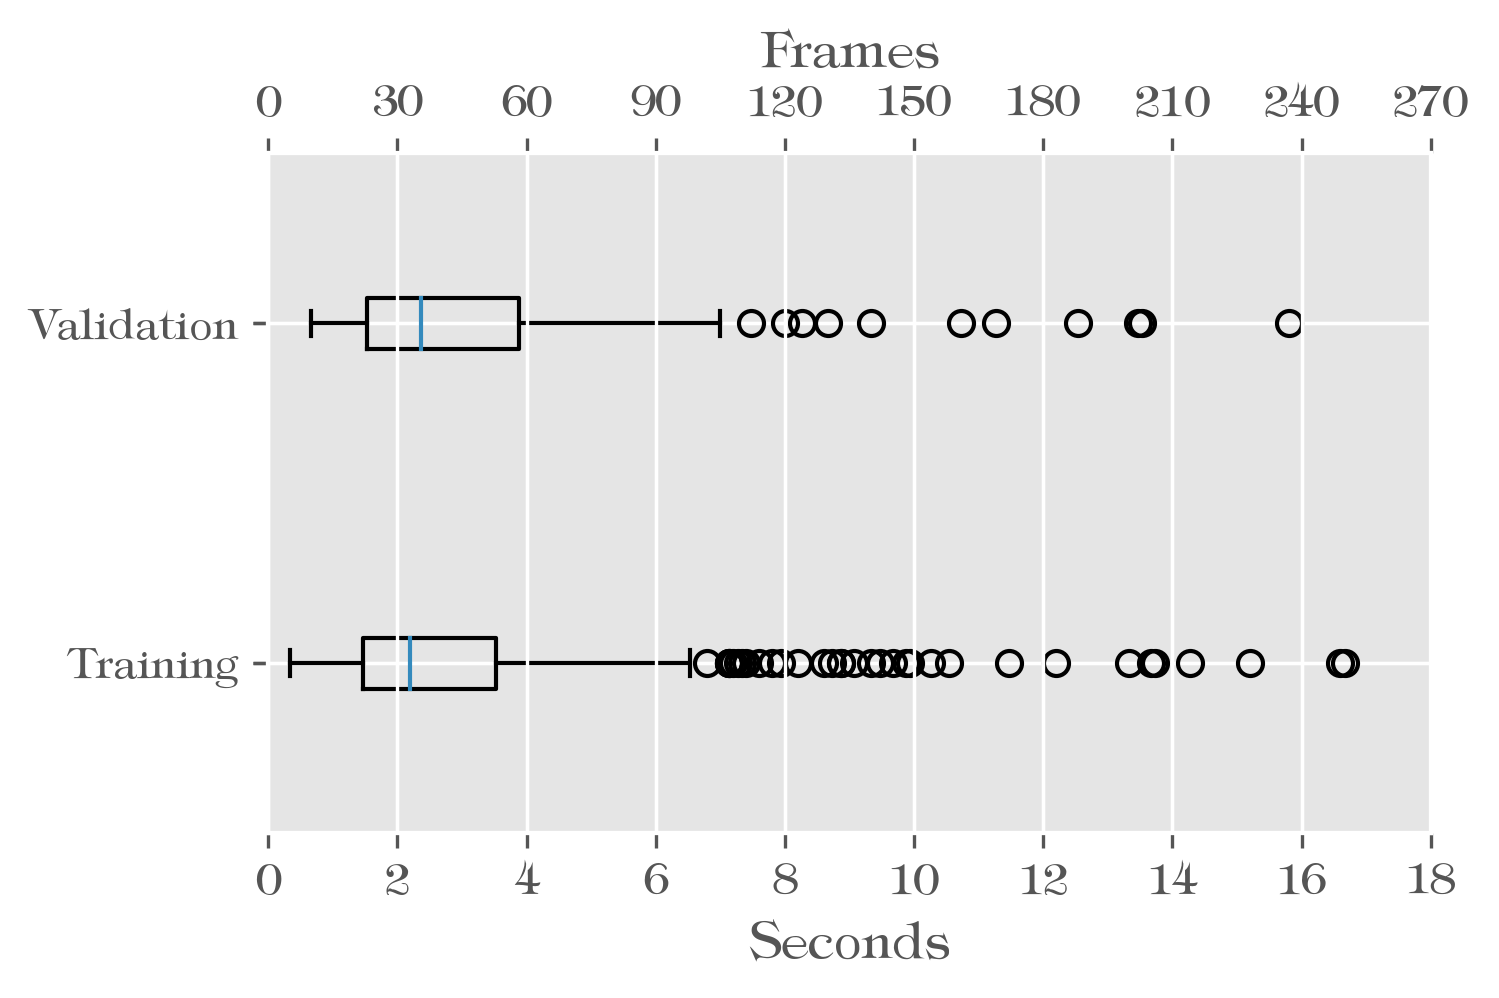
\includegraphics[width=\linewidth]{grafici/GTEA61_boxplot.png}		
	\end{center}
	\caption{GTEA-61 dataset; box-plots of sample lengths. A sample length is considered as outlier (and so represent as circle) if its value is greater than $Q_3 + 1.5(Q_3-Q_1)$, where $Q_i$ are quartiles}
	\label{fig:GTEA61_boxplot}
\end{figure}

The GTEA-61 dataset contains several video clips recorded at 15 fps which portray 7 common activities performed by 4 different subjects in a first person point of view. The actions are further divided into subcategories consisting in verb+object, such as \textit{open tea}, therefore totalling 61 different labels. In this work, we consider a constant split of the labelled data and we always consider the actions performed by subject 2 as validation data.

In figure \ref{fig:GTEA61_boxplot}, the distribution of the lengths of the video clips are represented by means of a pair of box-plots: as it can be seen, even though durations vary greatly, at least 75\% of both training and validation data is below 4 seconds. During our experiments we sample a fixed number of frames uniformly spaced in time. This means that for the great majority of the clips, the time span between two frames is a certain fraction of a second, ranging from approximately less than one-tenth to half a second. However, there are edge cases in which the time elapsed between two frames can be significantly higher or some other cases in which frames are being duplicated, as the case in which $N = 16$ frames are sampled but the clip is shorter than a second.

\subsection{Ego-RNN}

In this subsection, we present our experiments carried out on the models proposed in \cite{Ego-RNN}. In that work, two separate networks are proposed:
\begin{itemize}
	\item an RGB network, which consists of a ResNet backbone pre-trained on ImageNet, an attention mechanism, a ConvLSTM cell and a fully connected layer; the details of these blocks have been introduced in the previous paragraphs;
	\item a Flow Network, which consists of a ResNet backbone pre-trained on ImageNet
\end{itemize}

\subsubsection{RGB Network}

We trained the RGB network following the same 2-stage protocol and using the same hyperparameters of \cite{Ego-RNN}. However, we used a lower number of frames: we sampled $N = 7$ and $N = 16$ frames uniformly spaced in time.

We also replaced the attention mechanism with the one described in paragraph \ref{par:new_am}: to initialise the attention module, we sampled its weights from a normal distribution with $\mu = 0$ and $\sigma = .05$, which is close to be a Xavier initialisation; we obviously found out that missing this step and initialising the weights in a bad manner would almost completely cancel the performance boost given by this mechanism. We trained this new attention mechanism since stage 1, where instead the attention mechanism in \cite{Ego-RNN} is fine tuned only in stage 2.

\vspace{12pt} \noindent
\begin{tabular}{l|r}
	Network & Mean Validation Accuracy \\
	\hline
	RGB w/ NOCAM @ 7 & 54.31\% \\
	RGB w/ CAM @ 7 & 59.19\% \\
	RGB w/ NEW A.M. @ 7 & 59.90\% \\
	\hline
	RGB w/ NOCAM @ 16 & 56.32\% \\
	RGB w/ CAM @ 16 & 66.66\% \\
	RGB w/ NEW A.M. @ 16 & 65.51\% \\
\end{tabular} \vspace{6pt}

We can see that the new proposed attention mechanism works as effectively as the one proposed in \cite{Ego-RNN}. We think that this has partially to do with the given dataset: all samples share a very similar setting (a kitchen counter with almost always the same objects in the background across all scenes), and so, a stateless classifier is not capable of distinguishing one action from the other. As a result, the same neuron is used to compute the CAM among all scenes, hence why using one single neuron in the attention mechanism yields to the same results.

\subsubsection{Flow Network}

We trained the Flow network as done in \cite{Ego-RNN} using a single stack of 5 warp flow frames for each sample, and we got a mean accuracy of 40.52\% on the validation set. When we adopted the suggested validation strategy which consists in using 5 stacks of warp flow frames for each samples instead of 1, and then averaging the scores of the fully connected layer, we got a mean validation accuracy of 48.85\%, which is in line with the value reported in the original paper.

\subsubsection{Two-Stream}

Finally, following the same strategy and the same hyperparameters described in \cite{Ego-RNN}, we trained the two-stream model.

\vspace{12pt} \noindent
\begin{tabular}{l|r}
	Network & Mean Validation Accuracy \\
	\hline
	Two-stream @ 7 & 58.90\% \\
	Two-stream @ 16 & 75\%
\end{tabular} \vspace{6pt}

\subsection{Self supervised task}

We integrated the self supervised task on the second stage of the RGB network. We applied it on the output feature maps of the backbone, whose volume is 512x7x7: therefore, after resizing and cropping the generated IDT frame at the same location of the RGB frame, we downsampled it to 7x7 pixels.

For the motion segmentation task, we employed the following structure: the ReLu function is applied on the input; then a 1x1 convolution with 100 output planes, stride=1 and no padding, is applied; finally a fully connected layer is employed and it consists of 2 output neurons for each output pixel, i.e. a total of 98 output neurons.

We first adopted a 3x3 convolution, but the current input size is already small and so highly de-correlated, therefore using a 1x1 convolution makes more sense, and also yielded to better results. We first employed a dropout of 0.5 on the output fully connected layer: however, adopting a dropout on the output layer is discouraged and can lead to inaccurate predictions, since the correct output neurons can be prevented to fire; also, this branch is already simple and may not need this further regularisation even if applicable. 

Finally, we tried with one single output neuron for each pixel and minimised the Binary Cross Entropy Loss on the softmax of the output scores. ${BCE = y_i \cdot \log(x) + (1 - y_i) \cdot \log(1 - x_i), y \in \{0, 1\}}$ However, we obtain subpar results, and by using two output neurons for each output pixel, we obtained better results. This may have to do with the fact that, by increasing the size of the fully connected layer, the capacity of the network should increase as well, which may be beneficial in this instance; also, the BCE Loss suffers from numerical instability at certain values of the input, namely when it is close or equal to $0$ or $1$.

Therefore, as suggested in \cite{planamente2020joint}, we treated this auxiliary task as a classification task by computing the per-pixel cross entropy loss on the softmax of the output scores and we summed it to the main classification loss: ${L = L_{main} + \alpha L_{ms}, \alpha = 1}$.

\begin{figure}
	\begin{center}
		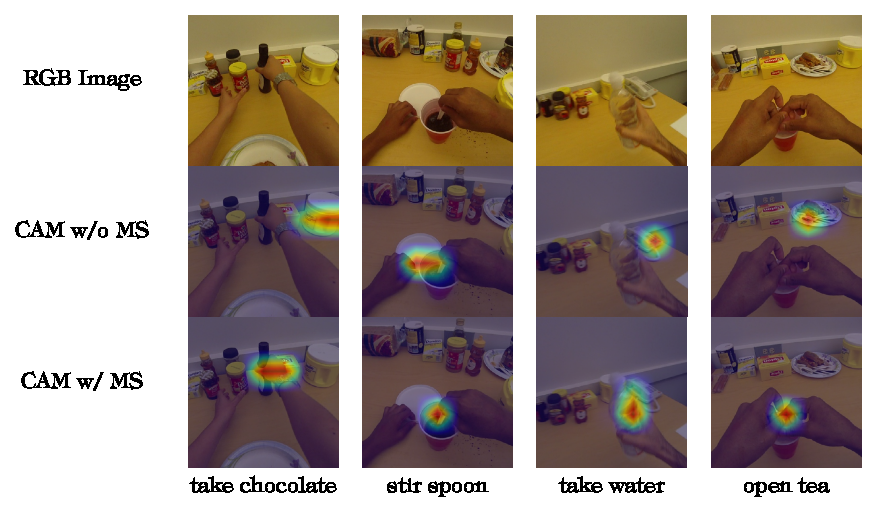
\includegraphics[width=\linewidth]{grafici/cams_img.pdf}		
	\end{center}
	\caption{Cam visualisations, before and after adding the MS task}
	\label{fig:cams}
\end{figure}

After adding the motion segmentation head on the second stage, we found out that the attention mechanism is more precise in certain scenes, such as the ones depicted in figure \ref{fig:cams}.

We also performed an hyperparameter optimisation: we trained for 150 epochs using Adam with a epsilon of 1e-4 and a batch size of 32, weight decay of 4e-5 and learning rate of 1e-4, which is divided by 10 after 25 and 75 epochs; for the auxiliary task, we experimented with different learning rates, weight decay and alpha, which is the multiplication factor of the loss of the auxiliary task, and with different numbers of frames.

As it can be seen from tables \ref{tab:ms_tb1} and \ref{tab:ms_tb2}, there is not a substantial change in accuracy when the factor alpha is changed; we observed a gain in accuracy when the number of frames was increased from 7 to 16 frames and when a low learning rate was lower. Due to the rather long training time, we skipped the value of 5 for alpha when doing 16 frames because setting that alpha seemed to be more counterproductive than anything when we tried with 7 frames.

\begin{table}[h!]
	\vspace*{0pt}
	\begin{center}
		\begin{tabular}{lcc|cc}
			\textbf{Alpha} & \textbf{Lr} & \textbf{Weight Decay} & \textbf{Loss} & \textbf{Accuracy [\%]}\\
			\hline
			0.5&0.001&1e-05&1.81&58.62\\
			0.5&0.001&4e-05&2.02&57.76\\
			0.5&0.005&1e-05&1.88&58.62\\
			0.5&0.005&4e-05&1.92&55.17\\
			0.5&0.01&1e-05&2.33&50.86\\
			0.5&0.01&4e-05&2.08&53.45\\
			1&0.001&1e-05&\textbf{2.11}&\textbf{60.34}\\
			1&0.001&4e-05&2.27&59.48\\
			1&0.005&1e-05&2.25&53.45\\
			1&0.005&4e-05&2.13&55.17\\
			1&0.01&1e-05&2.36&56.90\\
			1&0.01&4e-05&2.25&54.31\\
			5&0.001&1e-05&3.93&56.90\\
			5&0.001&4e-05&3.79&56.03\\
			5&0.005&1e-05&4.18&54.31\\
			5&0.005&4e-05&4.03&56.03\\
			5&0.01&1e-05&4.12&50.86\\
			5&0.01&4e-05&4.38&46.55\\
			\hline
		\end{tabular}
	\end{center}	
	\caption{Results with \texttt{CrossEntropyLoss} @ 7 frames}
	\label{tab:ms_tb1}
\end{table}

\begin{table}[h!]
	\begin{center}
		\begin{tabular}{lcc|cc}
			\textbf{Alpha} & \textbf{Lr} & \textbf{Weight Decay} & \textbf{Loss} & \textbf{Accuracy [\%]}\\
			\hline
			0.5&0.001&1e-05&1.63&66.38\\
			0.5&0.001&4e-05&1.69&63.79\\
			0.5&0.005&1e-05&1.61&65.52\\
			0.5&0.005&4e-05&1.62&65.52\\
			0.5&0.01&1e-05&1.76&68.10\\
			0.5&0.01&4e-05&1.54&65.52\\
			1&0.001&1e-05&1.87&66.38\\
			1&0.001&4e-05&\textbf{1.80}&\textbf{68.97}\\
			1&0.005&1e-05&1.90&62.07\\
			1&0.005&4e-05&1.90&62.93\\
			1&0.01&1e-05&1.81&63.79\\
			1&0.01&4e-05&1.96&63.79\\
			\hline
		\end{tabular}
	\end{center}	
	\caption{Results with \texttt{CrossEntropyLoss} @ 16 frames}
	\label{tab:ms_tb2}
	\vspace*{0pt}
\end{table}

\subsection{Self supervised as a regression problem}

In order to treat the self supervised task as a regression problem, we first replaced the activation function. Since two output neurons are employed for each pixel, their value are first summed. We then employed the $\tanh$ activation function since it can provide a steeper gradient than a sigmoid; however, when we squashed the value of $\tanh$ between 0 and 1, we did not observed any performance drop. Finally, we employed the mean square error loss: $ MSE = \frac{\sum_i (x_i - y_i)^2}{N}, y_i \in \{0, 1\}$. Again as before, we performed a grid search for the hyperparameters, and we can draw pretty much the same conclusions as of the classification variant.

\begin{table}[h!]
	\begin{center}
		\begin{tabular}{lcc|cc}
			\textbf{Alpha} & \textbf{Lr} & \textbf{Weight Decay} & \textbf{Loss} & \textbf{Accuracy [\%]}\\
			\hline
			0.5&0.001&1e-05&1.57&58.62\\
			0.5&0.001&4e-05&1.78&57.76\\
			0.5&0.005&1e-05&1.99&53.45\\
			0.5&0.005&4e-05&1.79&56.90\\
			0.5&0.01&1e-05&1.74&59.48\\
			0.5&0.01&4e-05&\textbf{1.72}&\textbf{61.21}\\
			1&0.001&1e-05&1.84&54.31\\
			1&0.001&4e-05&1.86&55.17\\
			1&0.005&1e-05&2.50&55.17\\
			1&0.005&4e-05&2.11&53.45\\
			1&0.01&1e-05&2.17&59.48\\
			1&0.01&4e-05&2.25&59.48\\
			5&0.001&1e-05&3.25&58.62\\
			5&0.001&4e-05&2.40&56.03\\
			5&0.005&1e-05&4.58&59.48\\
			5&0.005&4e-05&3.46&58.62\\
			5&0.01&1e-05&3.21&60.34\\
			5&0.01&4e-05&3.46&58.62\\
			\hline
		\end{tabular}
	\end{center}	
	\caption{Results with \texttt{MSRegressionClassificationLoss} @ 7 frames}
\end{table}

\begin{table}[h!]
	\begin{center}
		\begin{tabular}{lcc|cc}
			\textbf{Alpha} & \textbf{Lr} & \textbf{Weight Decay} & \textbf{Loss} & \textbf{Accuracy [\%]}\\
			\hline
			0.5&0.001&1e-05&1.51&62.93\\
			0.5&0.001&4e-05&1.67&61.21\\
			0.5&0.005&1e-05&1.70&65.52\\
			0.5&0.005&4e-05&1.63&64.66\\
			0.5&0.01&1e-05&1.72&65.52\\
			0.5&0.01&4e-05&1.60&68.10\\
			1&0.001&1e-05&1.68&63.79\\
			1&0.001&4e-05&\textbf{1.55}&\textbf{68.10}\\
			1&0.005&1e-05&1.64&67.24\\
			1&0.005&4e-05&1.78&65.52\\
			1&0.01&1e-05&1.66&65.52\\
			1&0.01&4e-05&1.64&68.10\\
			\hline
		\end{tabular}
	\end{center}	
	\caption{Results with \texttt{MSRegressionClassificationLoss} @ 16 frames}
\end{table}

\pagebreak

\subsection{Proposed method}

\subsubsection{Training WFCNet}

We trained WFCNet, i.e. the warp flow colorisation block, according to the protocol described in paragraph \ref{par:TrainingWFCNet}.

We used 7 frames/stacks for each sample: we experiment with either single warp flow frames and stacks of 5 warp flow frames. For the stage 1, we used the Adam optimizer with a batch size of 16, weight decay of 4e-5 and epsilon of 1e-4. We used a learning rate of 1e-2, which was multiplied by a coefficient .995 every epoch, we trained for 100 epochs. For the stage 2, we used the same hyperparameters, but we reduced the initial learning rate to 0.25e-4.

Again, we performed three runs for each variant, and for the next steps, we used the weights of the WFCNet blocks belonging to the best performing runs.

\begin{figure}
	\begin{center}
		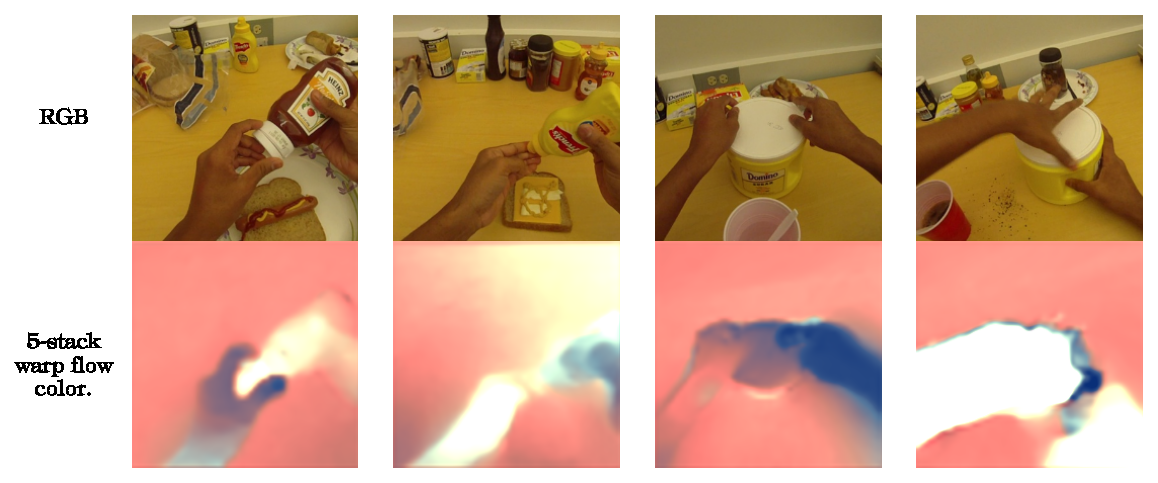
\includegraphics[width=\linewidth]{grafici/wfcnet_color_img.pdf}		
	\end{center}
	\caption{Warped optical flow colorisation performed on stacks of 5 warp flow frames}
	\label{fig:wfcnet_color_img}
\end{figure}

In figure \ref{fig:wfcnet_color_img}, we show what the WFCNet block produces when it is applied to stacks of 5 consecutive warped optical flow frames: we can see that still objects are removed and melted in a single-colour background, and only hands, arms and moving objects are retained. Furthermore, fast moving objects appear to be brighter than slowly moving objects; however, given that an RGB frame is produced from 5 consecutive warp flow frames, fast movements may be represented inaccurately: as showcased in the last sample, the hands of the subject and the manipulated object bleed into a single bright blob, making the action recognition more challenging than desired.

\subsubsection{RGB Network with colorised warp flow frames}

In order to train the RGB network with colorised warp flow frames, we followed the same strategy described in paragraph \ref{par:our_rgb_network}. Specifically, for stage 1 we used the Adam optimizer with a batch size of 32, weight decay of 4e-5 and epsilon of 1e-4.  We used a learning rate of 1e-2, which was divided by 10 after 50 and 100 epochs. We trained for 120 epochs. For stage 2, we lowered the initial learning rate to 1e-4 and we divided it by 4 at epochs 30, 50 and 75; we trained for 120 epochs.

\vspace{12pt} \noindent
\begin{tabular}{l|r}
	Network & Val. Accuracy \\
	\hline
	WFCNet single -> RGBNet @ 7 & 26.43\% \\
	WFCNet single -> RGBNet @ 14 & 28.16\% \\
	\hline
	WFCNet stack of 5 -> RGBNet @ 7 & 35.34\% \\
	WFCNet stack of 5 -> RGBNet @ 14 & 33.04\% \\
\end{tabular} \vspace{6pt}

The results are underwhelming: the warp flow frames are somehow useful to classify the action, but either the loss in resolution and detail is too dramatic to confidently classify the involved action or our proposed network can not exploit the warp flow frames up to their full potential.

We also acknowledge that our results are inferior to the ones obtained with the temporal network proposed in \cite{Ego-RNN}: our hypothesis is that, by training the whole network as it is done \cite{Ego-RNN}, greater results can be achieved than just fine tuning the last layer of the backbone as it is done in this RGB network.

\subsubsection{Two-input network}

We finally tested our two-input network. In the first stage, we used the Adam optimizer with a batch size of 32, weight decay of 4e-5 and epsilon of 1e-4; we used a learning rate of 1e-3, which was halved after 50 epochs; we trained for 100 epochs. We trained the second stage for 100 epochs, we lowered the initial learning rate to 1e-4 and we halved it after 50 epochs.

\vspace{12pt} \noindent
\begin{tabular}{l|rr}
	Network & Stage 1 & Stage 2 \\
	\hline
	Stack of 5 + RGB @ 7 & 52.58\% & 63.22\% \\
    Stack of 5 + RGB @ 14 & 60.34\% & 71.83\% \\
\end{tabular} \vspace{6pt}

As it can be seen from the reported results, our two-input variant is able to achieve interesting results: despite being unable of reaching high performances, we believe that our method can exploit warped optical flow in a more effective manner. For instance, while in Ego-RNN there is a substantial accuracy drop when the number of frames is halved, which somehow suggests that probably the ``heavy-lifting'' of the action recognition task is to be attributed to the RGB information, our proposed two-input network is able to maintain an above-60\% accuracy even at 7 frames at the end of the second stage.

\begin{figure}[h!]
	\begin{center}
		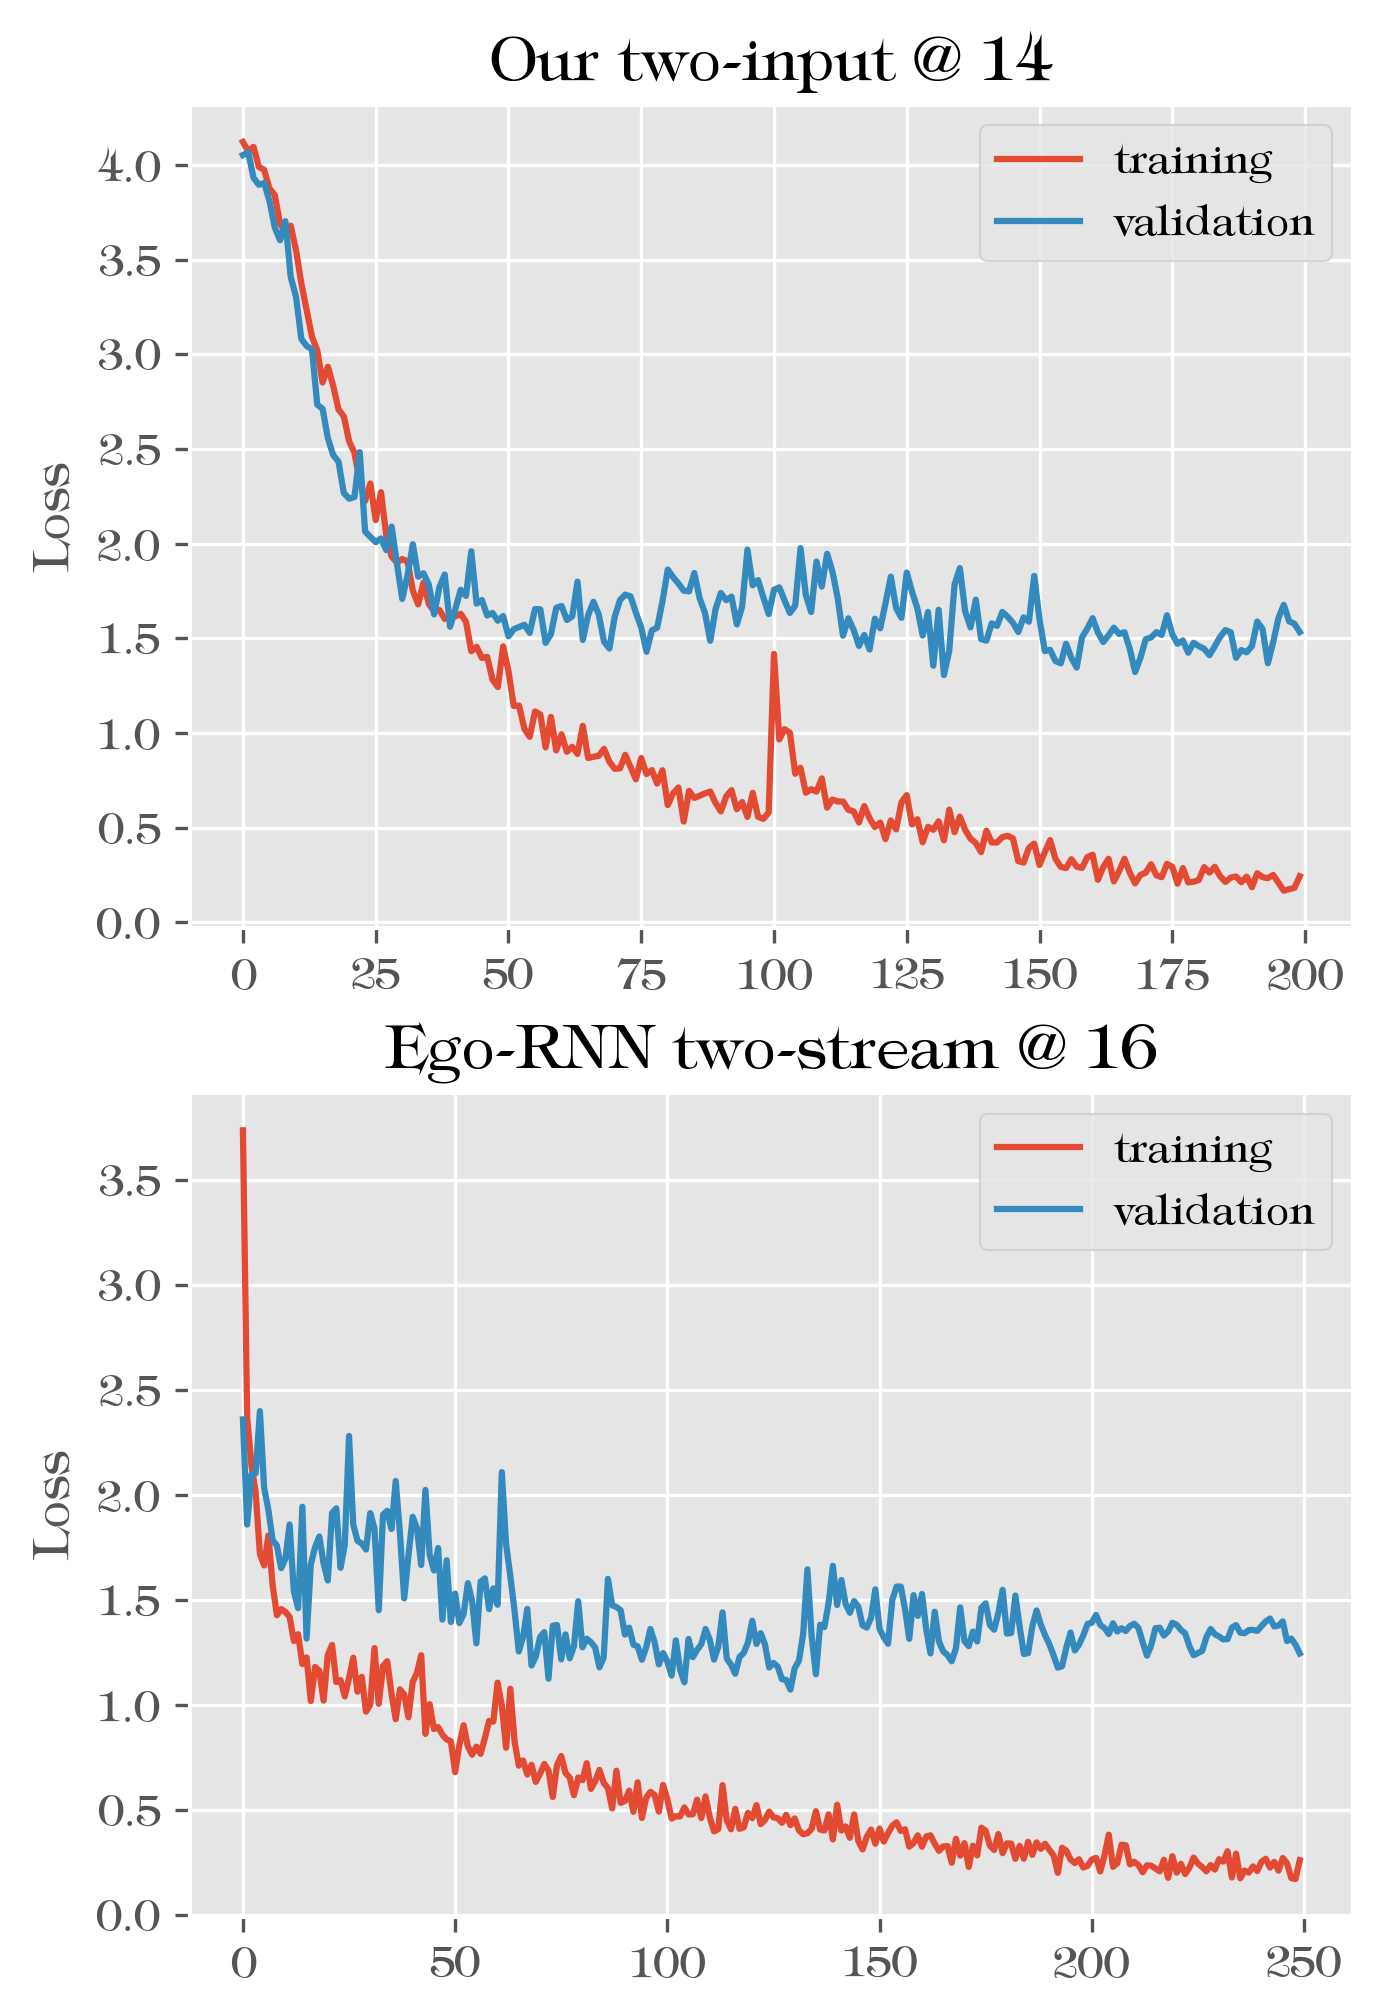
\includegraphics[width=\linewidth]{grafici/losses.png}		
	\end{center}
	\caption{}
	\label{fig:losses}
\end{figure}

However we want to point out one last remark: both our proposed variant and the two-stream model of Ego-RNN exhibit a certain overfitting on the training data as proved by the gaps between training loss and validation loss as shown figure \ref{fig:losses}: so a performance drop is not unimaginable on a more diverse dataset, such as EPIC-KITCHENS-100, hence why probably an higher number of frames may be required to reach the same performances on those more challenging datasets.

\section{Conclusions}

In our work we presented a number of techniques for tackling the first person action recognition task. We first presented the capability of the attention mechanism in boosting the overall performances without requiring a complete retraining of the backbone, and we then later showed how a simpler attention mechanism can be employed without hindering the overall performances. After showcasing the performances achieved by a two-stream model, we experimented with the potentialities offered by self-supervision, which in particular involved an auxiliary task on IDT maps and whose aim is to remove the need of training on optical flow frames. We then decided to further experiment with warp flow frames: by our experimentations, we found out that warp flow frames may not be sufficient alone to solve the given problem, but when instead they are coupled with RGB frames, some interesting results can be achieved.

We finally point out that our proposed models are not production ready: for instance, we found out that the action can be partially occluded by the central square crop, and therefore we suggest to employ at least a better dimensioned backbone, capable of accepting 16 by 9 frames rather than square frames.

{\small
\bibliographystyle{ieee_fullname}
\bibliography{egbib}
}

\end{document}
